%
% Spark refernce architectures
% Copyright (C) 2016 Jan Machacek
%
% This program is free software: you can redistribute it and/or modify
% it under the terms of the GNU General Public License as published by
% the Free Software Foundation, either version 3 of the License, or
% (at your option) any later version.
%
% This program is distributed in the hope that it will be useful,
% but WITHOUT ANY WARRANTY; without even the implied warranty of
% MERCHANTABILITY or FITNESS FOR A PARTICULAR PURPOSE.  See the
% GNU General Public License for more details.
%
% You should have received a copy of the GNU General Public License
% along with this program.  If not, see <http://www.gnu.org/licenses/>.
%

\documentclass[a4paper, 10 pt, conference]{IEEEtran}

\usepackage{graphicx}
\usepackage{interval}
\usepackage{listings}
\usepackage{hyperref}
\usepackage{siunitx}
\usepackage{amsmath}

\sisetup{load-configurations = abbreviations, binary-units = true}
\intervalconfig {
soft open fences ,
separator symbol =; ,
}

\title{Spark Reference Architecture \\ Connected home}

\author{Jan Mach{\'a}\v{c}ek%$^{1}$% <-this % stops a space
%\thanks{Supported by Cake Solutions Limited}% <-this % stops a space
%\thanks{$^{1}$J. Machacek is the CTO at Cake Solutions, Houldsworth Mill, Houldsworth Street, Reddish, SK5 6DA, UK {\tt\small janm at cakesolutions.net}}%
}


\begin{document}

\maketitle
\thispagestyle{empty}
\pagestyle{empty}

%%%%%%%%%%%%%%%%%%%%%%%%%%%%%%%%%%%%%%%%%%%%%%%%%%%%%%%%%%%%%%%%%%%%%%%%%%%%%%%%
\begin{abstract}

TODO

\end{abstract}


%%%%%%%%%%%%%%%%%%%%%%%%%%%%%%%%%%%%%%%%%%%%%%%%%%%%%%%%%%%%%%%%%%%%%%%%%%%%%%%%
\section{Introduction}

TODO

\section{Reference implementation}

This year appears to be the perfect time to start building internet-of-things platforms: the availability of sensors has never been greater, while their cost has never been lower. Together with wide availability of smart hubs?devices that provide screen-less access to the nearby devices?and our prediction that these devices will provide local platform for the IoT devices, there will be growing need to build larger cloud-based applications that ingest the data, contextual information, and commands from the applications on these smart hubs.
Such cloud-based application needs to be able to handle significant volume of incoming data in a reliable and responsive manner. The responsiveness and reliability expectations for the applications for the smart hubs far exceed those of ordinary web or mobile applications: the users are even less likely to tolerate delays or failures. 
The Lightbend stack, with help from Kafka, Apache Spark and Mesos are the perfect choices to implement the cloud-based portion of such a system. The application you see implements the crucial elements of an IoT platform: the ingestion service receives the data from the hubs and sensors. It then reconstructs the messages, checks their integrity and authenticity, decodes the payloads, and passes the data on to Kafka to deliver the payloads to the subscribed microservices. The back-pressure reporting is used to ensure that the infrastructure can flex up or down to deal with the load. Kafka (with Zookeeper) allows us to reason about the order of messages, the delivery guarantees; these then serve as constraints on the implementation of the microservices. Using this architecture, it is possible to clearly separate the ingestion / storage microservices from the streaming and batch analytics services. \autoref{fig:ri-architecture} illustrates the main components and the sizes of the data flows; it leaves out the infrastructural concerns.

\begin{figure}[h]
	\begin{center}
		\caption{Architecture}
		\label{fig:ri-architecture}
		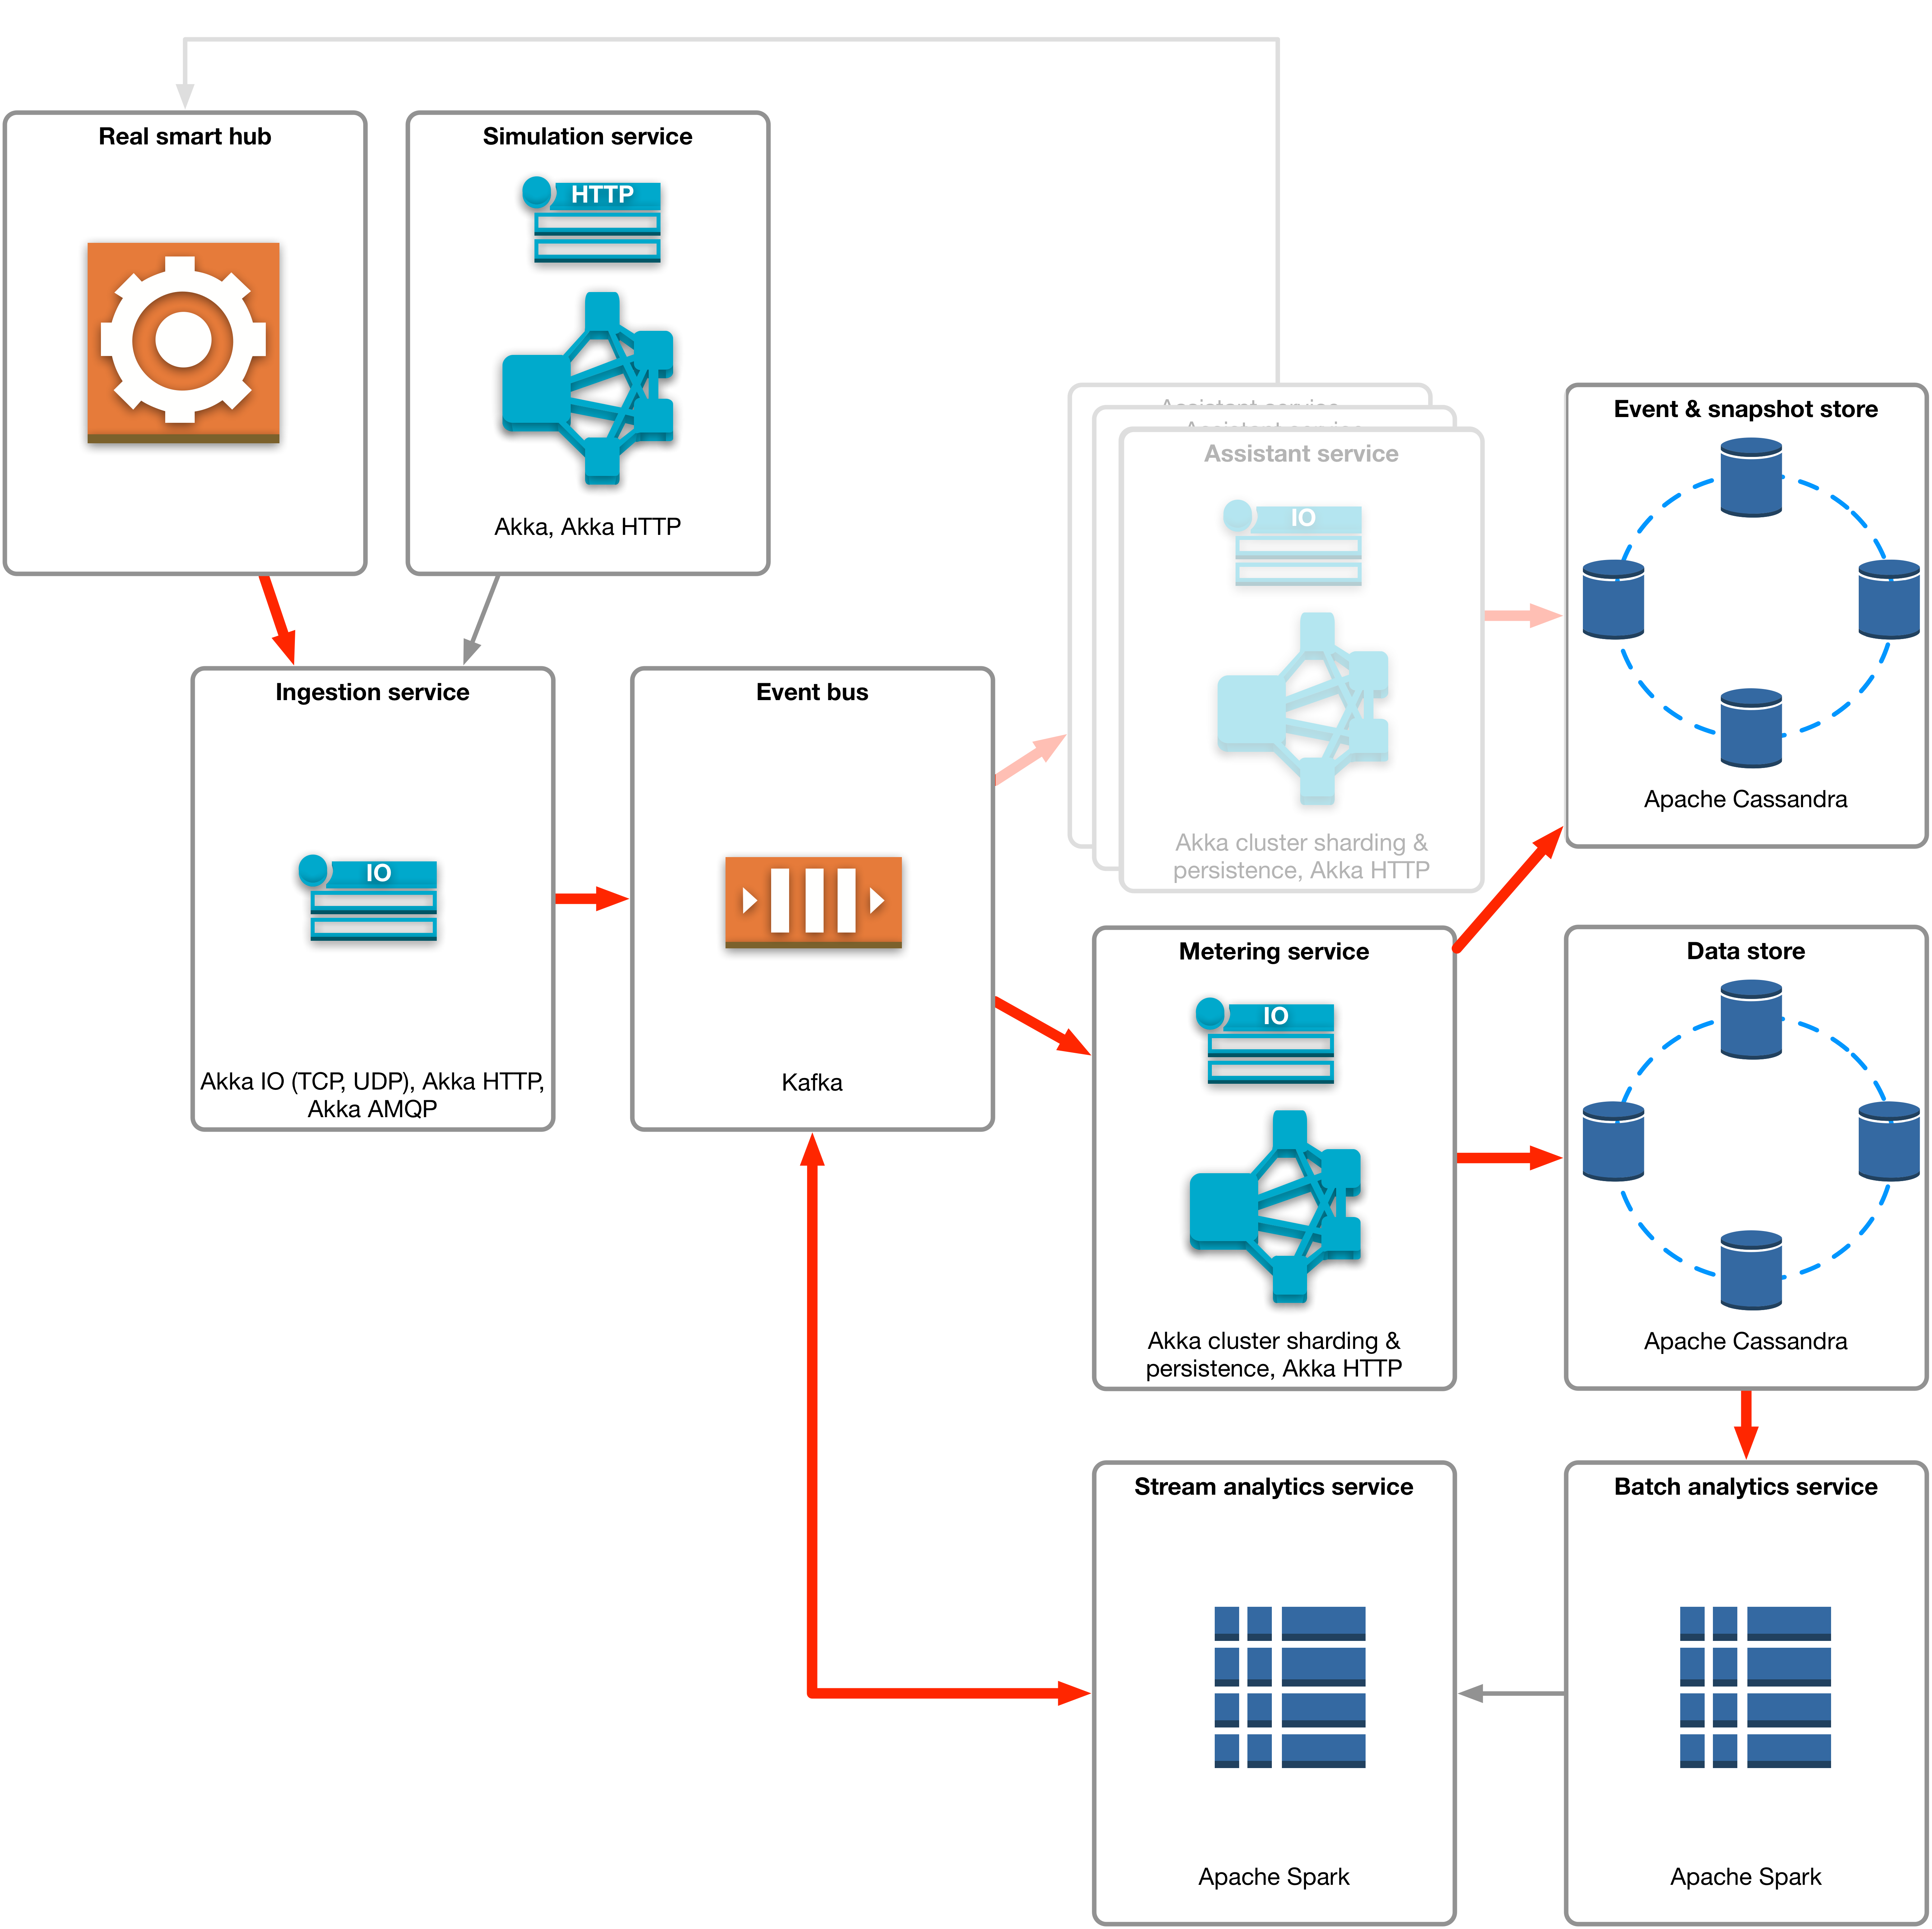
\includegraphics[width=7cm,keepaspectratio]{ri-arch.png}
	\end{center}
\end{figure}

\section{Infrastructure}

To run this application, the infrastructure needs to be able to make the most of the available computing resources (CPU, GPU, RAM, storage, etc.) and to provide sufficient service discovery functionality; it must also provide sufficient monitoring and log management. The monitoring components need to be able to trigger scale up or down as necessary, the triggers in this type of architecture are typically back-pressure indicators. The main infrastructure components are shown in \autoref{fig:ri-infrastructure}.

\begin{figure}[h]
	\begin{center}
		\caption{Infrastructure}
		\label{fig:ri-infrastructure}
		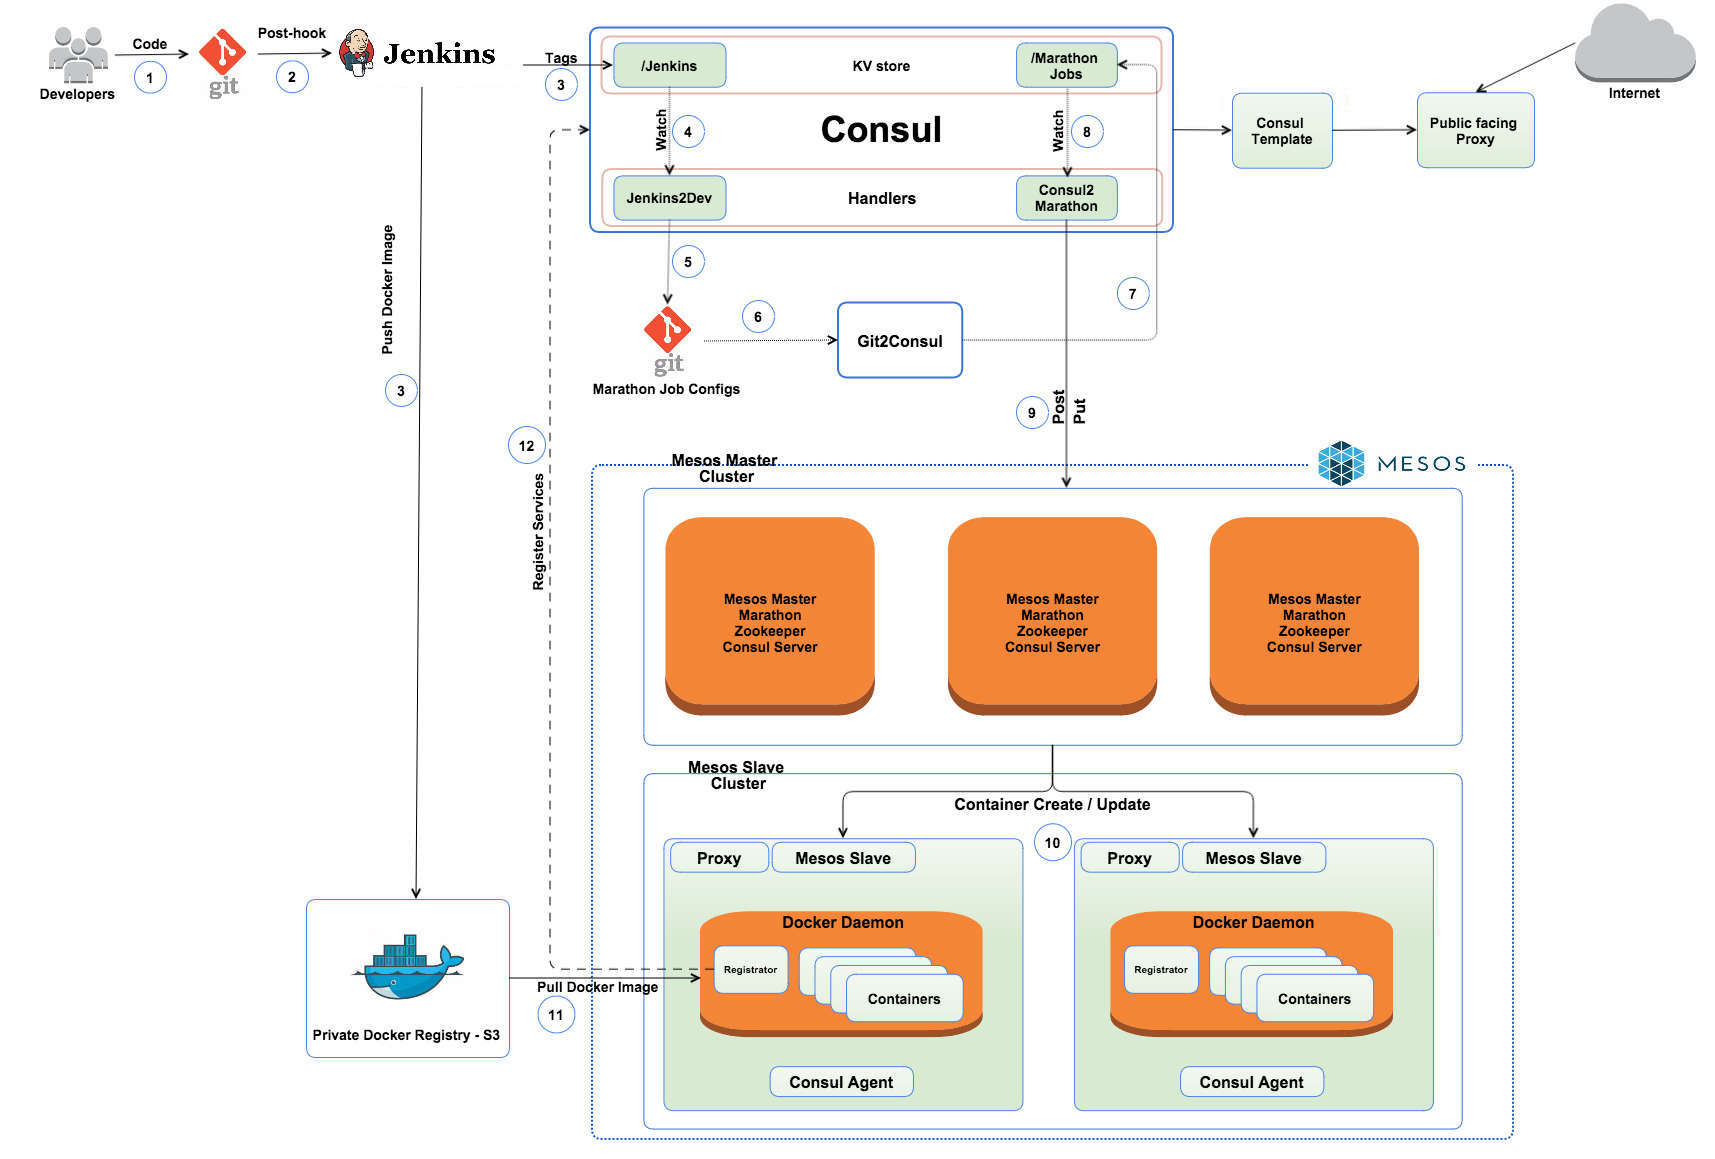
\includegraphics[width=7cm,keepaspectratio]{ri-infrastructure.jpg}
	\end{center}
\end{figure}


\section{Summary}

\addtolength{\textheight}{-12cm}  % This command serves to balance the column lengths
                                  % on the last page of the document manually. It shortens
                                  % the textheight of the last page by a suitable amount.
                                  % This command does not take effect until the next page
                                  % so it should come on the page before the last. Make
                                  % sure that you do not shorten the textheight too much.

\begin{thebibliography}{99}

\bibitem{x} X.

\end{thebibliography}


\end{document}
